\section{Research}\label{research}




\noindent The main focus of this report is to prevent injury to a person jumping on a trampoline. In order to do so, examination of existing safety issues and common avoidance methods has been carried out to expand this understanding. In addition to this, analysis of the mechanics of the trampoline itself is important and will help enable understanding of when a dangerous situation can arise. Knowledge of these factors will enable a model to be created that is as true to life as possible.  


\subsection{Trampoline Safety}\label{trampsafety}


% \\
% \\
% \noindent As seen in Figure \ref{fig:injuries} below taken from the

% \begin{figure}[H]
% 	\centering
% 	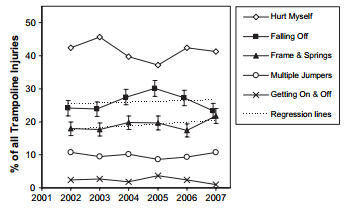
\includegraphics[width=0.6\linewidth, height=1.6in]{injuries.png}
% 	\caption{(cite Report)}\label{fig:injuries}
% \end{figure}

\noindent The Leisure Safety Information published by the Royal Society for the Prevention of Accidents (RoSPA) in 2007 states some advice guidelines and facts for parents who are worried about the safety of their children on trampolines \cite{rospa}. The most common protective additions to a trampoline are safety pads and netting enclosures. Safety pads, which are impact resistant foam covered in PVC  used to cover the springs on the edge of the trampoline, are essential in preventing injury and require little maintenance to be effective. Without these covers, limbs could get trapped between the frame of trampoline and the springs leading to bruising injuries or injuries such as fractures or breaks from a harsh landing onto the springs or frame. A netting, if of appropriate height, will prevent users bouncing off of the trampoline and therefore preventing any injury. As shown in the 2011 AvonSafe summary on trampoline injuries \cite{actionforsafety}, a lack of a safety net results in a 64\% higher injury outcome, from the Ninewells Hospital study.  Use of both these pieces of equipment will minimise the risk of injury to users in accordance with adult supervision and appropriate use of the trampoline. 
\\
\\
\noindent In regards to multiple users, both AvonSafe and RoSPA suggest this is the largest cause of injury in trampoline use, with 80\% and 74\% prevalence of injury respectively \cite{actionforsafety}. The only possible responses in order to prevent or reduce these injuries is to either allow only one person on the trampoline at a time, or to look at the interaction between multiple users on the trampoline and observe when this interaction will result in injury. It is therefore possible to  offer guidance on how multiple users should use the trampoline. This is investigated in Section \ref{results}.
\\
\\
\noindent It has also been advised by a combination of the manufacturers, the USA Consumer Safety Council and RoSPA that children under the age of six should not be allowed on trampolines of sizes greater than 20 inches in height or a diameter greater than ten feet \cite{rospa}. This is a response suggested as young children are lightweight and have not the necessary motor coordination skills required for good stability on a trampoline.
\\
\\
The location of the trampoline is also important as poor placement can contribute to safety issues. A recommendation from RoSPA is that the trampoline should be placed on soft energy absorbing ground, such as a lawn or bark wood chip \cite{rospa}. The area should also be clear of hazardous objects, such as trees, fences and washing lines. The impacts on different surfaces will be investigated in Section \ref{futureinjury}.

\subsection{Physics of a Trampoline}


%	Transfer of energy
\noindent It is important to look at the transfer between the kinetic and potential energies of a person bouncing on a trampoline. Consider a single mass dropped onto a trampoline. When it comes into contact with the trampoline from being dropped, the trampoline will extend down to a point. Ascending from this position, the mass loses kinetic energy and gains potential energy, the combination of these two is the total energy of the mass \cite{physics}. \\

\noindent When an overlap occurs in the time two masses dropped onto the trampoline are in contact with the trampoline then there is a transfer in energy between them and the mass dropped second will `absorb' the first mass' energy, resulting in a higher bounce \cite{physics}, whilst the first simultaneously has no energy left to bounce back upwards.
\\
\\%	Balanced forces?
\noindent The elastic nature of the trampoline itself must also be investigated to understand how it contributes to increasing a person or objects height in a bounce. The springs in the trampoline are subject to Hooke's Law, stating that the force needed to compress or stretch a spring by some distance is proportional to that distance \cite{physics}. Therefore the springs will attempt to return to equilibria position, producing a reaction force that propels the object or person back upwards. 
\\
\\
%Newtons laws?
The person bouncing upon the trampoline has their movement dictated by Newton's second law, that the forces acting upon an object are dependent on the mass and acceleration of said object \cite{nasa}. Thus, the force that the trampoline exerts on each mass creates an acceleration, which causes the mass to increase in velocity, and rise above the trampoline until the velocity is decreased to zero, due to the acceleration of gravity, and the mass begins its descent. %change first sentance